\documentclass[a4paper,11pt,final]{report}

\usepackage[english,francais]{babel}
\usepackage[utf8]{inputenc}
\usepackage[T1]{fontenc}
\usepackage[pdftex]{graphicx}
\usepackage{setspace}
\usepackage{hyperref}
\usepackage[french]{varioref}
\usepackage[final]{pdfpages}
\usepackage{titlesec}
\usepackage{minted}

\graphicspath{{images/}}

\newcommand{\reporttitle}{Ordonnancement dans des systèmes distribués}
\newcommand{\reportauthor}{Teddy \textsc{Gilbert} Simon \textsc{Espigolé} Hugo \textsc{Legrand}}
\newcommand{\reportsubject}{Rapport de projet GSI}
\newcommand{\HRule}{\rule{\linewidth}{0.5mm}}
\setlength{\parskip}{1ex}

\titleformat{\chapter}[display]
  {\normalfont\bfseries}{}{0pt}{\huge}

\hypersetup{
    pdftitle={\reporttitle},
    pdfauthor={\reportauthor},
    pdfsubject={\reportsubject},
    pdfkeywords={rapport} {vos} {mots} {clés}
}

\author{ESPIGOL\'{E} Simon & GILBERT Teddy & LEGRAND Hugo}

\begin{document}

\begin{titlepage}

\begin{center}

\begin{minipage}[t]{0.48\textwidth}
  \begin{flushleft}
    
\includegraphics [width=30mm]{images/logo_eisti.jpg} \\[0.5cm]
    \begin{spacing}{1.5}
      \textsc{\LARGE}
    \end{spacing}
  \end{flushleft}
\end{minipage}
\begin{minipage}[t]{0.48\textwidth}
  \begin{flushright}
  \end{flushright}
\end{minipage} \\[1.5cm]

\textsc{\Large \reportsubject}\\[0.5cm]
\HRule \\[0.4cm]
{\huge \bfseries \reporttitle}\\[0.4cm]
\HRule \\[1.5cm]

\begin{minipage}[t]{0.3\textwidth}
  \begin{flushleft} \large
    \emph{Étudiants :}\\
    \reportauthor
  \end{flushleft}
\end{minipage}
\begin{minipage}[t]{0.6\textwidth}
  \begin{flushright} \large
    \emph{Responsable :} \\
    Juan Angel \textsc{LORENZO DEL CASTILLO} \\
  \end{flushright}
\end{minipage}

\vfill

{\large Pau, le \today}

\end{center}

\end{titlepage}


\chapter{Remerciements}
Nous voudrions remercier Juan Angel \textsc{Lorenzo Del Castillo}, pour son aide et ses conseils précieux lors des différentes séances de programmation ainsi que durant les cours qu'il nous a enseigné.

Aussi nous remercions Rémi \textsc{Vernay} pour ses différents cours d'algorithmique et programmation parallèle qui nous ont permis de mieux comprendre ce projet et comment l'implémenter.


\tableofcontents


\newpage

\chapter{Introduction}
    \section{Définition du sujet}
    
    L'ordonnanceur (\texttt{scheduler}, en anglais) est l'élément central d'un système d'exploitation multi-processus. L'ordonnancement (\texttt{Scheduling}) définie une méthode par laquelle un travail, \texttt{work}, va être attribué à un processeur pour une partie ou pour la totalité de son fonctionnement. Un ordinateur disposant de ressources limitées et un travail nécessitant des ressources pour fonctionner (puissance de calcul, capacité mémoire, etc...), l'ordonnanceur doit savoir répartir ces travaux afin d'optimiser les ressources matérielles à disposition du système. Il peut avoir plusieurs objectifs : 
    
    \begin{itemize}
        \item Optimisation du nombre de travaux complétés par unité de temps (\texttt{Maximize throughput})
        \item Minimiser le temps de réponse d'un processus en particulier (\texttt{Latency})
        \item Minimiser le temps d'attente des programmes dans la file d'attente (\texttt{Responsiveness})
        \item Égaliser les ressources disponibles pour chaque processus (\texttt{Fairness})
        \item etc...
    \end{itemize}
    
    Il est très difficile d'implémenter un ordonnanceur capable d'optimiser plusieurs aspects à la fois. Par exemple, il faut faire un compromis entre le nombre de travaux complétés et le temps de réponse d'un processus en particulier (\texttt{Throughput} VS \texttt{Latency}). De plus, chaque optimisation de l'ordonnanceur correspond à une stratégie d'ordonnancement spécifique et peut avoir de sérieuses conséquences sur la stabilité et les performances du système d'exploitation.
    
    \section{Contexte et objectif}
        
    Dans le cadre du Projet GSI de seconde année d'ingénieur, nous avons réalisé un scheduler permettant d'ordonnancer différents processus selon une certaine stratégie d’ordonnancement. À réaliser en équipe de 3 personnes, nous avons utilisé les méthodes vues en cours pour développer ce projet, qui nous a permis d'apprendre la programmation C++ et la programmation parallèle. De plus, pour la première fois notre outil de gestion de version de code (GitLAB) a été accessible par le responsable du projet, nous avons donc du adapter nos commits à cette situation, les décrire d'une façon plus claire, mais surtout utiliser une convention de nommage comme suit :
    
    \begin{itemize}
        \item Séparer le sujet du corps avec un saut de ligne
        \item Limiter le sujet à 50 caractères
        \item Mettre une majuscule au premier mot du sujet
        \item Ne pas finir le sujet par un point
        \item Utiliser l'impératif pour le sujet
        \item Limiter le corps à 72 caractères par ligne
        \item Utiliser le corps pour expliquer quoi, pourquoi et comment
    \end{itemize}
    
    Nous avons donc essayé d'aller au-delà des attentes classiques d'un projet Eistien pour avoir une approche encore plus professionnelle du projet informatique.

\chapter{Présentation de l'interface utilisateur}

    Nous avons choisi une interface en ligne de commande pour ce projet. En effet, nous avons préféré nous investir dans le fond et terminer un maximum de fonctionnalités plutôt que de passer du temps sur une interface graphique dont l'intérêt pour un projet comme celui-là reste limité. L'interface présentée est celle de l'ordonnanceur séquentiel.

    \vfill
    \begin{figure}[!h]
        \centerline {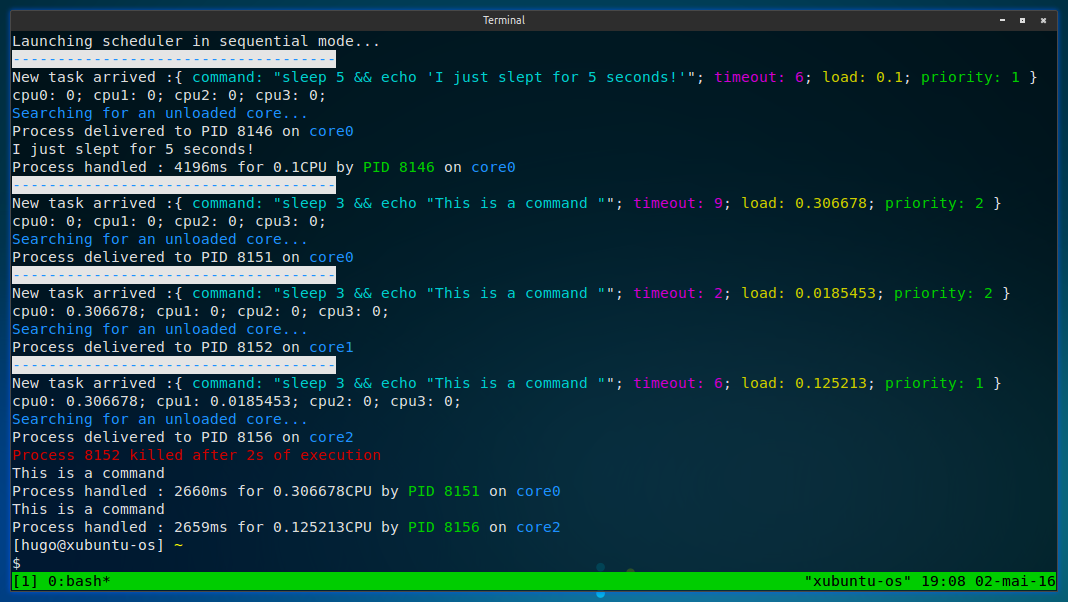
\includegraphics[scale=0.5]{images/scheduler-s.png}}
        \caption{Affichage sheduler du programme}
        \label{Affichage scheduler du programme}
    \end{figure}
    
    \begin{figure}[!t]
        \centering
        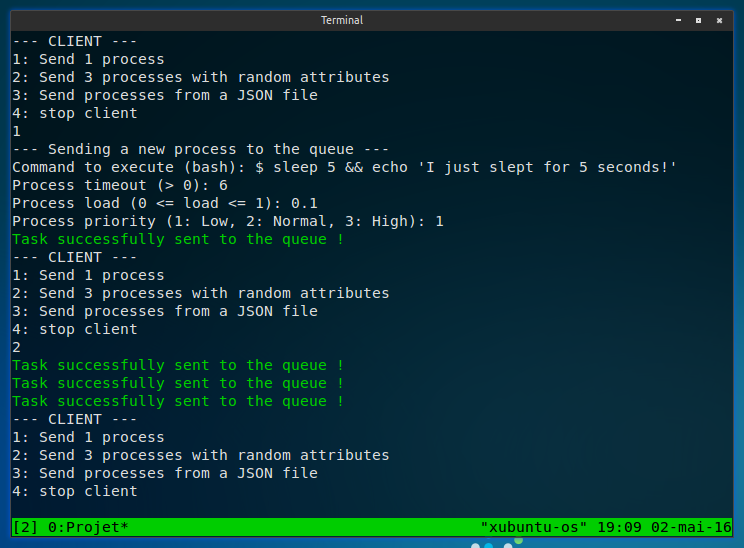
\includegraphics[scale=0.5]{images/scheduler-c.png}
        \caption{Affichage client du programme}
        \label{Affichage client du programme}
    \end{figure}

    Après avoir lancé le scheduler puis le client sur deux émulateurs de terminal différents, l'utilisateur interagit avec le client avec quatre menus principaux :
    
    \begin{itemize}
        \item Send 1 process
        \item Send 3 processes with random attributes
        \item Send processes from a JSON file
        \item Stop client
    \end{itemize}
    
    Il est intéressant de noter que l'ordre de lancement entre les deux programmes importe peu. En revanche, le fait de quitter le client n'arrête pas le scheduler. Lorsque le client est quitté, il faudra attendre que le scheduler s'arrête\footnote{Voir 5.1 Lancement du programme et timeout} (ou l'arrêter de manière brutale). En effet, le canal de communication est ouvert indifféremment pas les deux programmes mais est fermé par le client. Cela est du à une volonté de notre part de pouvoir manipuler le scheduler (démarrage, arrêt, coupure brutale) d'une façon très fluide. \newline
    
    Si l'utilisateur choisit la première option (Send 1 process), alors il lui sera demandé plusieurs attributs à remplir pour que sa tâche soit envoyée au scheduler. Notamment : 
    
    \begin{itemize}
        \item La commande à exécuter (en bash)
        \item Le temps d'expiration (timeout) de la commande (en secondes)
        \item La charge de cette commande sur un processeur (entre 0 et 1)
        \item La priorité de la tâche (entre 1 et 3)
    \end{itemize}
    
    Si la commande à exécuter n'est pas interprétable par un shell, le programme quittera.
    Après avoir remplit tous ces attributs, le client envoie la tâche au scheduler qui la traitera selon notre stratégie d'ordonnancement\footnote{Voir Chapitre 4 Stratégie d’ordonnancement} puis imprime le message suivant à l'écran : "Task successfully sent to the queue !". 
    
    Si l'utilisateur choisit la seconde option (Send 3 processes with random attributes), le client va afficher les tâches qu'il va envoyer au scheduler : "created : { command: "sleep 3 \&\& echo "This is a command ""; timeout: 2; load: 0.627926; priority: 2 }", les envoie au scheduler puis affiche le message suivant : "Task successfully sent to the queue !".
    
    Les résultats seront alors visibles sur l'écran du scheduler qui affiche son traitement comme suit, pour chaque tâche arrivée :
    
    \vbox{
    \begin{verbatim}
------------------------------------
New task arrived :{ command: "sleep 3 && echo "This is a command"";
    timeout: 10; load: 0.960486; priority: 1}
cpu0: 0; cpu1: 0; cpu2: 0; cpu3: 0;
Searching for an unloaded core...
Process delivered to PID 10359 on core0
This is a command // Ici la commande est exécutée.
Process handled : 3010ms for 0.960486CPU by PID 10359 on core0
    \end{verbatim}
    }
    
    En outre, le client peut charger un fichier JSON à partir de la troisième option. Il lui faudra juste préciser le chemin ainsi que le nom du fichier à partir du dossier d'exécution du programme.
    
    Si tout le fichier est écrit correctement alors les messages suivant s'afficheront après la demande du fichier. Si une tâche ne possède pas la bonne syntaxe, la lecture de fichier s'arrêtera et affichera une erreur. 
    
    \vbox{
    \begin{verbatim}
--- Enter the path of json file  ---
test.json
Task successfully sent to the queue !
Task successfully sent to the queue !
....
Task cannot be created. Verify your json file.
    \end{verbatim}
    }

Voici un template de fichier JSON que notre programme pourra analyser. Si jamais il manque un argument(command,timeout,load,priority) le programme entrera lui même l'argument manquant. Cela ne produira pas d'erreur et sera totalement transparent. 

    \vbox{
    \begin{minted}{json}
{
  "0" :{
    "command":"sleep 3 && echo \"This is a command\"",
    "timeout":10,
    "priority":3
  },
  "1":{
    "command":"sleep 3 && echo \"This is a command\"",
    "load":0.5,
    "priority":1
  },
  "2" :{
    "command":"sleep 3 && echo \"This is a command\"",
    "timeout":1,
    "load":0.7,
    "priority":2
  },
  "3" :{
    "command":"sleep 3 && echo \"This is a command\""
  },
  "4" :{
    "command":"sleep 3 && echo \"This is a command\"",
    "timeout":2,
    "load":0.98,
    "priority":3
  }
}
    \end{minted}    
    }
    
    Le scheduler peut aussi afficher d'autres messages différents, mis dans le désordre ici, qui seront détaillés plus tard :
    
    \vbox{
    \begin{verbatim}
...
Process 10359 killed after 2s of execution // Voir 4.4.2 Expiration d’une tâche
...
No unloaded core found ! // Voir 4.1 Algorithme 
Searching for a core that can fit the task...
...
    \end{verbatim}
    }

\chapter{Stratégie d'ordonnancement}

   \section{Algorithme}
    
    Concernant l'algorithme d'ordonnancement utilisé, nous avons décidé de développer notre propre solution. Dans la section suivante, nous expliquerons pourquoi avoir fait ce choix. Voici la traduction en pseudo-code :
    
    \begin{verbatim}
    TANT QUE non timeout FAIRE
        -- Une nouvelle tâche arrive
        SI aucun processeur ne peut contenir la tâche
            Attendre qu'un processeur se libère
        SINON
            SI un processeur est vide (pas de tâches en cours)
                lui attribuer automatiquement la tâche.
            SINON
                Récupérer le processeur le moins utilisé
                Lui assigner la tâche
            FINSI
        FINSI
    FIN TQ
    \end{verbatim}
    
    \section{Choix de la stratégie}

    Notre stratégie d'ordonnancement dérive de l'une des stratégies les plus répandues : \texttt{Load balancing} + FIFO. Cette stratégie implémente le principe d'une file d'attente. Le premier processus arrivé est affecté\footnote{\textsc{FIFO}: \texttt{First In First Out}}. \newline 
    Bien que relativement simple, cette solution a pour avantage de garder les ressources occupées et de ne pas surcharger un processeur grâce à la répartition des charges. \newline
    
    Le développement de notre propre algorithme de \texttt{scheduling} nous a permis d'inclure certaines optimisations et fonctionnalités supplémentaires. Nous détaillerons ces fonctionnalités dans la section \textsc{Optimisation de l'ordonnancement}.
    
    Il est intéressant de noter que notre ordonnanceur vise en priorité les processeurs vides afin d'affecter une tâche. Nous avons donc une optimisation horizontale de la charge CPU. Cela diffère d'une optimisation verticale qui recherche à mettre le maximum de ressources sur un processeur avant de passer au suivant. 
    
    \underline{Raison} : Il nous semble plus intéressant de chercher à paralléliser le plus possible les processus afin de gagner en temps d'exécution plutôt qu'à optimiser les ressources dans un système quasiment non contraint en CPU. De ce fait, nous utilisons toute la puissance disponible sur la machine.\newline
    
    
    \section{Implémentation}
    
    Afin de pouvoir doter le programme d'une interface utilisateur fluide, nous avons opté pour une architecture \texttt{Client-Serveur}. Le client\footnote{Le client s'exécute avec la commande Scheduler -c (ou --client)} permet de remplir la file de message de plusieurs manières\footnote{Cf. \textsc{Présentation de l'interface utilisateur}}. L'utilisation de la file de message permet d'avoir un canal de communication quasi-instantanée entre le client et l'ordonnanceur tout en ne consommant que très peu de ressources (dû à son implémentation très bas niveau en C).\newline
    
    Le serveur\footnote{Le serveur s'exécute avec la commande Scheduler -s pour le mode séquentiel ou Scheduler -p pour le mode parallèle}, séquentiel ou parallèle, lit tous les messages de la file de messages, selon leur ordre d'arrivée (FIFO).
    
    
    \subsection{En parallèle}
    
    Notre \texttt{scheduler} dispose d'un mode parallèle. Dans ce mode, certaines opérations d'ordonnancement ont été optimisées avec la librairie \texttt{OpenMP} afin de réduire le temps entre le moment où une tâche arrive et le temps où elle est affectée à un processeur. \newline
    
    Les fonctions paralèllisées sont les suivantes : 
    
    \begin{itemize}
        \item Recherche d'un processeur capable de contenir la tâche
        \item Recherche d'un processeur vide
        \item Recherche du processeur le moins chargé
    \end{itemize}
    
    Il est important de noter que la file de message de l'ordonnanceur reste la même quelque soit le mode. Il est donc tout à fait possible de traiter quelques tâches en mode séquentiel, d'arrêter le programme et de le relancer en mode parallèle afin de terminer les affectations.\newline
     
    Malgré nos efforts d'implémentation, il ne s'agit pas réellement d'un \texttt{scheduler} parallèle. En effet, les tâches ne sont pas affectées à un processeur de manière simultanée mais seulement quelques opérations de recherche ont été optimisées.
    
    \section{Optimisation de l'ordonnancement}
    
    Comme précisé précédemment, le développement de notre propre algorithme d'ordonnancement nous a permis d'y inclure quelques fonctionnalités supplémentaires. Ces améliorations sont disponibles en mode séquentiel et parallèle.
    
    \subsection{Tâches prioritaires}
    
    Lorsque l'utilisateur crée une tâche, il doit lui affecter une priorité\footnote{Cf. \textsc{Présentation de l'interface utilisateur}}. Cette priorité permet à l'ordonnanceur de savoir que la tâche doit être affecté le plus rapidement possible. Ainsi, dans la file de message, le \texttt{scheduler} cherchera toujours à assigner la plus ancienne tâche (arrivée la première) avec la priorité la plus élevée.
    
    \subsection{Expiration d'une tâche}
    
    Nous avons implémenté un système permettant de tuer une tâche trop longue à s'exécuter. En effet, si le temps d'exécution \textbf{réel} dépasse le \texttt{timeout}\footnote{Cf. \textsc{Présentation de l'interface utilisateur}}, la tâche expire et est tuée par l'ordonnanceur. \newline
    
    Cette méthode n'est pas une étape en plus dans la boucle\footnote{Cf. \textsc{Algorithme}} pour le \texttt{scheduler} car elle ne s'exécute pas dans le \texttt{thread} principale du programme. En effet,  elle est encapsulée dans l'exécution de la tâche elle-même, ce qui permet la libération de charges sur le CPU tout en continuant l'affectation. Pour schématiser, son comportement est semblable à une tâche qui détecterait elle-même qu'elle dépasse le temps que le processeur lui avait accordé et se "suiciderait".  Cette fonctionnalité, d'une extrême simplicité, est très efficace et permet de simuler l'ordonnancement dans un système contraint en temps.
    
    \subsection{Historique de session}
    
    Bien que ce ne soit pas une optimisation d'ordonnancement (car cela n'améliore pas les performances du \texttt{scheduler}), le programme dispose d'un journal contenant l'historique de sa dernière utilisation. Ceci permet d'analyser le comportement de l'ordonnanceur sans avoir à garder un terminal ouvert. Le journal se situe à l'endroit depuis lequel le programme est exécuté.

\chapter{Déroulement du programme}

    \section{Lancement du programme et timeout}
    
    Au lancement du programme scheduler, un temps d'expiration (timeout) est lancé. Passé ce timeout, le programme quittera automatiquement. Le timeout est de 60 secondes au lancement du programme, et est relancé à chaque tâche reçue par le scheduler pour la valeur du timeout de la tâche entrée par l'utilisateur auquel nous additionnons 60 secondes. L'utilisateur a donc en moyenne une minute pour interagir avec le programme avant que celui-ci ne quitte.
    Si le programme scheduler quitte, le relancer suffira pour de nouveau interagir avec le programme client, même si celui-ci n'a pas été fermé.

    \section{Remplissage de la file de message}
    
    Afin que l'ordonnanceur puisse travailler, il faut tout d'abord remplir la file avec des tâches à consommer. Pour cela, exécuter le programme en mode client :
    
    \begin{verbatim}
        $ ./Scheduler --client
    \end{verbatim}
    
    Puis choisissez le mode d'envoi des messages que vous souhaitez. Vous pouvez laisser le client ouvert et continuer à envoyer des tâches dans la file pendant l'exécution de l'ordonnanceur. Ne pas oublier d'ouvrir un scheduler :
    
    \begin{verbatim}
        $ ./Scheduler --sequential
        $ ./Scheduler --parallel
    \end{verbatim}

    

    \section{Workflow}
    
    \vfill
    \begin{figure}[!b]
        \centerline {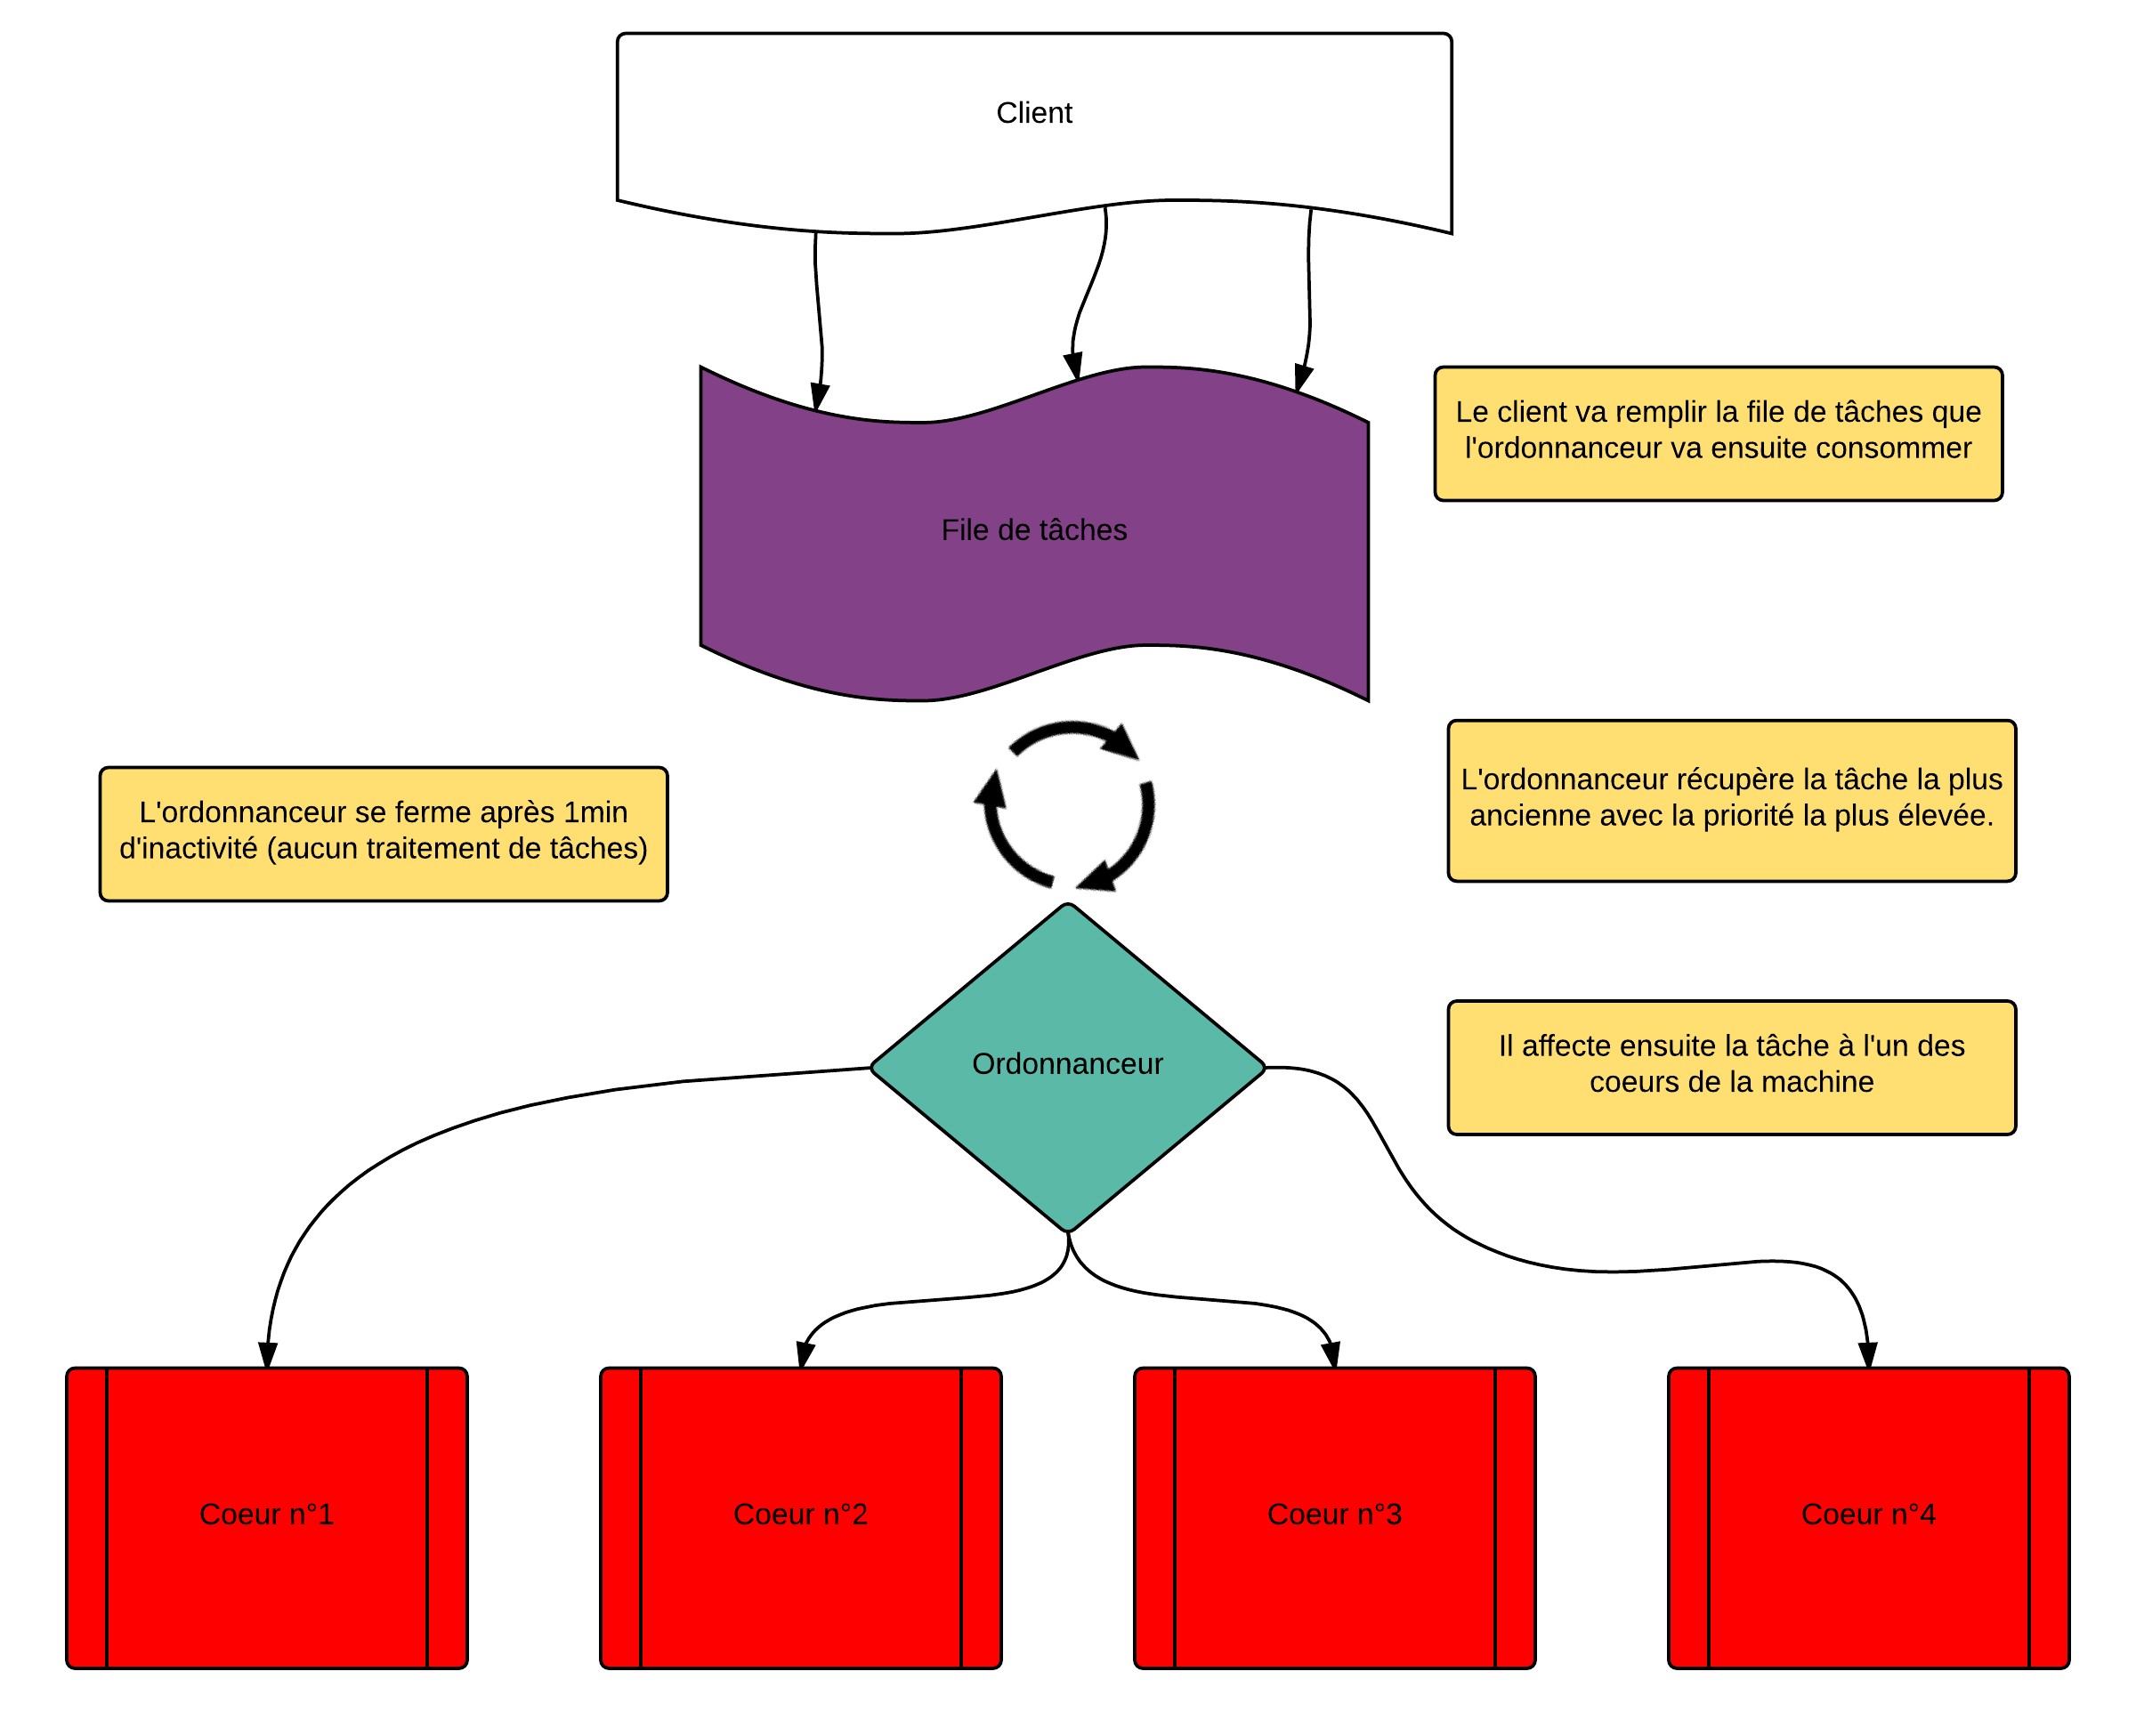
\includegraphics[scale=0.22]{workflow.png}}
        \caption{Workflow (happy path) de notre programme}
        \label{Workflow (happy path) de notre programme}
    \end{figure}

\chapter{Problèmes rencontrés}

Pendant le développement de ce projet, nous avons chacun rencontré différents problèmes. Heureusement composé de trois membres, notre groupe a su répondre aux problématiques de chacun de ses membres en s'entraidant dans les difficultés rencontrées par tous les protagonistes. En outre, cette entraide nous a permis de mieux cerner le sujet mais aussi mieux comprendre les enjeux de la parallélisation.

\section{Processus zombies}

    Du fait de la parallélisation, nous avons connu quelques problèmes avec les processus zombies. En effet, nous lançons la commande demandée par l'utilisateur sur un processus nouveau, ce qui nous permet de la contrôler entièrement (finir son exécution ou la tuer). Or, certains processus restaient en mode zombie plutôt que de se terminer proprement. Après quelques recherches, nous avons trouvé la solution en faisant comme suit :

    \vbox{
    \begin{minted}{c}
        if (exec == 0) {
            setpgid(getpid(), getpid());
            std::system(command.c_str());
            ...
            exit(EXIT_SUCCESS);
        } else {
            sleep(_task.timeout);
            pid_t result = waitpid(exec, &status, WNOHANG);
            // If his child is still alive...
            if (result == 0) {
                // Kill the process because the timeout is exceeded
                kill(-exec, SIGTERM);
                ...
            }
        }
    \end{minted}
    }
    
    En effet, pour terminer un fils proprement, il faut envoyer le signal \textsc{EXIT\_SUCCESS}. Le père, si le timeout est dépassé, va récupérer le signal de fin d'exécution du fils avec la commande \textsc{waitpid}. Si le résultat vaut 0 (signal renvoyé si le fils est toujours en vie), alors le père va décider de le tuer avec la commande \textsc{kill(-exec, SIGTERM)}. Il faut noter que le "-" placé devant le PID "exec" permet de rendre le PID négatif et donc de tuer tous les processus associés au groupe de processus ayant pour PGID "exec". Le PGID est défini grâce à la ligne \textsc{setpgid(getpid(), getpid());}.

\section{Portée des variables et accès concurrents}

    L'une des premières difficultés lors de l'exécution parallèle des tâches a été la portée des variables du programme. En effet, lors d'un \texttt{fork}, les variables communes entre le processus père et son fils ne sont pas partagées mais copiées. Précisément, un fils a accès aux variables de son père mais leur contexte reste celui juste avant le \texttt{fork}. De ce fait, le père ne peut en aucun cas avoir connaissance des changements apporter par son fils sur ces variables. Pour y faire face, nous les avons placées à l'intérieur de conteneur, des \texttt{Shared Memory}. En procédant de cette manière, plusieurs processus peuvent lire et modifier une même variable à travers un programme. \newline
    
    Cependant, la lecture et l'écriture simultanée d'une variable, d'un fichier texte ou d'une structure entraîne des accès concurrents. Nous avons dû sécurisé ces opérations grâce à des \texttt{mutex}. Il s'agit d'un système de jeton permettant de restreindre l'accès d'un objet à un seul et unique processus à un instant t.

    

\section{Parallélisation et échange de variables}
    
    Lors de la parallélisation du scheduler, nous avons rencontré plusieurs problèmes de concurrences. Tout d'abord, en appliquant une simple parallélisation des boucles for pour la recherche du CPU. Un problème est alors survenu sur la charge des CPU. Ils dépassaient leur charge possible (>1). Il a fallu partager avec un \textsc{\#pragma omp shared} les boucles afin d'éviter ce problème.
    
    De plus, lors de la recherche d'un CPU libre, la boucle for se coupait si l'un des CPU était libre. Or en parallélisation, cela n'est pas possible. Donc nous avons rajouté une variable de stockage. Puis à la fin de la parallélisation, nous avons fait une somme logique grâce au \textsc{\#pragma omp reduction}. 
    
    Pour finir, un problème venait de la parallélisation des affectations. Cela n'est pas possible hormis si nous mettions un endroit critique afin que tous les threads n'affectent pas leur valeur en même temps. Cette fonction est donc restée non parallèle. Ce sont les limites de la parallélisation. 
    
\section{Problèmes liés à l'horloge}

    Lors de l'implémentation d'une horloge pour mesurer le temps d'exécution réel d'une commande passée par l'utilisateur, nous avons remarqué que pour une commande censée durer 5 secondes, l'horloge nous affiche un temps de 4100ms à 4900ms environ. En effet nous pensons que cela est dû au temps d'initialisation de l'horloge, qui varie selon l'exécution.
    Nous n'avons cependant pas trouvé de solution à cette problématique.

\chapter{Critique du module}

    \section{Compréhension}
    
    Le projet de simuler un \texttt{scheduler} est très intéressant. Cela nous a permis de comprendre un peu plus comment fonctionnait l'ordonnancement des tâches sur un ordinateur. Le sujet a été très clair concernant les technologies à utiliser et les modalités de livraison. Cependant, nous regrettons un certain flou par rapport à la limite qui différenciait l'ordonnanceur séquentiel de l'ordonnanceur parallèle.
    
    \section{Organisation du projet}
    
    L'organisation des groupes était très bien car nous avions le choix d'être avec les personnes que nous voulions. Il est vrai que des groupes imposés aurait fortement handicapé et ralenti un projet dont les délais étaient déjà assez court. \newline
    
    Un des problèmes était qu'au début du projet nous ne connaissions rien et nous avons fait les cours en parallèle. Nous ne pensons pas que cela soit une bonne stratégie. Certes, les compétences sont mises directement en application mais le projet avance moins vite et c'est un peu plus brouillon. Le fait d'avoir les connaissances au début du projet nous aurait permis de ne pas faire d'erreur au départ et d'avoir un planning à long terme. Il a fallu plusieurs fois modifier le code car il ne correspondait plus à ce que nous pouvions ni devions faire.

\chapter{Conclusion}

    Ce projet a été pour nous une source d'apprentissage inconsidérable. Ce dernier nous a permis de mieux comprendre une grande partie des matières enseignées au second semestre. De plus, il a été un support pour ces matières tout au long de cette période. Il a été parfois difficile de rester en phase avec les cours puisque nous avions besoin de plus de matériel pour continuer à travailler sur le projet.
    
    Bien qu'il fut compliqué de comprendre au départ les subtilités de ce projet, nous avons réussi en un temps raisonnable à nous approprier ce dernier et commencer à faire les premières fonctionnalités. 
    
    Nous avons, selon nous, fait un travail de qualité sur ce projet en nous concentrant sur un code propre, bien écrit, commenté, documenté (grâce à doxygen), et respectant un maximum de normes de bon sens. De plus, nous nous sommes efforcés de faire des commits utiles sur Git, pour une compréhension accrue de notre repository.
    
    Pour toutes ses raisons, nous pensons avoir réussi notre projet sur la forme en premier lieu puisque nous avons fait de notre mieux pour nous engager dans une démarche sérieuse et professionnelle. Bien sûr, nous avons aussi appris de ce projet sur cette démarche et savons ce que nous devrons refaire et ce que nous ne devrons pas
    
    En conclusion, nous avons tenté de mêler technique et gestion de projet, en utilisant un maximum de connaissances qui nous ont été enseignées durant nos différentes années d'études à l'EISTI, et sommes fiers du résultat obtenu. De plus, nous avons trouvé ce sujet très intéressant puisque techniquement élevé et aimerions retravailler sur un projet de ce type à l'avenir.

\chapter{Bibliographie}

\begin{itemize}
    \item \url{http://bisqwit.iki.fi/story/howto/openmp/}
    \item \url{http://www.boost.org/doc/libs/1_60_0/}
    \item \url{http://man7.org/linux/man-pages/man2/sched_setaffinity.2.html}
\end{itemize}

\begingroup
\let\clearpage\relax
\listoffigures
\endgroup


\end{document}


% TODO
%  6.2 Portée des variables et accès concurrents (problems_encountered)
%  Critiques du module